\documentclass[../Languages.tex]{subfiles}

\begin{document}
\usec{Lisp}\label{sec:lisp}

\cd{Lisp} (historically, \cd{LISP}) is a family of computer programming
languages with a long history and distinctive, fully parenthesized prefix
notation. Originally specified in 1958, \cd{Lisp} is the second-oldest
high-level programming languages in widespread use today. Only
\cd{Fortran} is older, by one year. \cd{Lisp} has changed since
its early days, and many dialects have existed overs its history. Today, the
best known general-purpose \cd{Lisp} dialects are \textit{Common Lisp} and
\textit{Scheme}.

\cd{Lisp} was originally created as a practical mathematical notation for
computer programs, influenced by the notation of Alonzo Church's lambda
calculus. It quickly became the favored programming language for artificial
intelligence (AI) research. As one of the earliest programming languages,
\cd{Lisp} pioneered many ideas in computers sciences, including tree data
structures, automatic storage management, dynamic typing, conditionals,
higher-order functions, recursion, the self-hosting compiler, and the
read-eval-print loop.

The name \cd{\textit{LISP}} derives form ``LISt Processor''. Linked lists
are one of \cd{Lisp}'s major data structures, and \cd{Lisp} source code
is made of lists. Thus, \cd{Lisp} programs can manipulate source code as a
data structure, giving rise to the macro systems that allow programmers to
create new syntax or new domain-specific languages embedded in \cd{Lisp}.

The interchangeability of code and data gives \cd{Lisp} its instantly
recognizable syntax. All program code is written as s-expressions, or
parenthesized lists. A function call or syntactic form is written as a list
with the function or operator's name first, and the arguments following; for
instance, a function \mintinline{lisp}{f} that takes three arguments would be
called as \mintinline{lisp}{(f arg1 arg2 arg3)}.

\subsection{Influence}\label{sub:influence}

\begin{Figure}
  \centering
  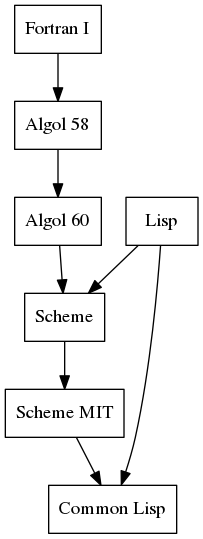
\includegraphics[height=0.5\textheight]{lisp}
  \captionof{figure}{Inheritance diagram for \cd{Lisp}.}
\end{Figure}

\newpage
\end{document}
